\chapter{Results}
\label{chap:results}

In this chapter the results of the GraphSLAM algorithm are presented for different test scenarios. In section~\ref{sec:known-asso-res} the algorithm is tested for the simple case of known data association and simulated data. A parameters variation analysis is made, and their effect in the path estimation is shown. In section~\ref{sec:unknown-asso-res} a similar analysis is performed, but for the case of unknown data association. In this case, new parameters related to the data association algorithm are tested. Finally in section~\ref{sec:real-data-res}, the GraphSLAM algorithm is run in more realistic data. This data includes robot simulated with Gazebo\footnote{http://gazebosim.org/}, a much more realistic robot simulator, and data obtained from real robots in outdoor environments. 

Through this tests several parameters and methods must be chosen for the algorithm to work properly. To limit the scope of this work, the sparse solver and the optimization algorithm are fixed and used in all the following tests. CSpase library and the Cholesky decomposition is used for the sparse solver, and the Levenberg-Marquardt method is used as the optimization algorithm. Also whenever the robust kernel method is used, Huber is the chosen kernel function (see section~\ref{sec:known-asso-imp}). 

\section{Known Data Association}
\label{sec:known-asso-res}

The known data association case is the easiest one of the three scenarios, because correspondence between landmarks is given a priori. In this case the user must simply set the parameters and run the solver as stated in Algorithm~\ref{alg:known-correspondence}. 

The parameters to be set in this case are the following:

\begin{itemize}
    \item $n_p$: number of poses of the robot path.
    \item $n_l$: number of landmarks in the map.
    \item $i_{op}$: odometry position information (inverse of variance).
    \item $i_{oa}$: odometry angle information.
    \item $i_{lp}$: landmark position information.
    \item $it$: number of iterations for the optimization algorithm to stop.
    \item $k_w$: Width of the chosen robust kernel.
\end{itemize}

Where $n_p$, $n_l$, $i_{op}$, $i_{oa}$, and $i_{lp}$ are parameters regarding the robot behavior in the test. They are passed to the simulator. The parameters $it$ and $k_w$ define de optimization strategy.

Through all the test made in this work, it is assumed that the information matrix of odometry and measurements models (same as~\eqref{eq:info-matrices}) are diagonal, i.e., their variables are not correlated. Furthermore, it is assumed that these matrices have the following structure:

\begin{equation}
\bs{R}^{-1}_k = \begin{pmatrix}
i_{op} & 0 & 0\\
0 & i_{op} & 0\\
0 & 0 & i_{oa}
\end{pmatrix} \;\;
\bs{Q}^{-1}_k = \begin{pmatrix}
i_{lp} & 0\\
0 & i_{lp}
\end{pmatrix} 
\label{eq:info-matrices-tests}
\end{equation}

This means that the robot experiences same uncertainty in the $x$ and $y$ axis, for both, motion and measurement model. 

\nameref{sec:test-i} is run with the parameters of Table~\ref{tab:test-i}. 

The simulation is constrained to a 2D world with $x\in[-15,15]$, $y\in[-15,15]$. At each step the simulator moves the robot 1 unit of distance and in turns randomly an angle of $\theta=0^\circ$, $90^\circ$, or $-90^\circ$. All simulations start from at $(0,0)$.

A kernel width of 1 unit is chosen heuristically, looking at the distance between landmarks. 

The results of the test are shown in Figure~\ref{fig:test-i}. In Figure~\ref{fig:test-ia} the initial guess is plotted on the left, and the posterior estimation after the solver on the right. The groundtruth is added in both graphs for comparison. Landmarks not observed by the robot are not shown.  It can be seen that the path of the initial guess rapidly diverges from the real solution. On the other hand, the solver estimation fits quite well with the groundtruth, both for the path and the landmarks.

To have a more quantitative view of the error made by the solver, the cumulative path error for every step is shown in Figure~\ref{fig:test-ib}.  The cumulative normalized error is given by:

\begin{equation}
error (i) = \frac{1}{i} \sum_{i} ||pos_{GT}-pos_{est}||
\end{equation} 

Where $i$ is the path's timestep. $pos_{GT}$ and $pos_{est}$ are the groundtruth and estimated position respectively. Then the error is the sum of the euclidean distance of both positions, normalized by the number of steps. 

It can be seen that the error start increasing early in the path, but then it get stabilized. This is the effect of aggregating the information of the measurements and running the optimizer. As long as the robot keep measuring the same landmarks, it can maintain its error low. 


\subsubsection{Test I.}
\label{sec:test-i}

\begin{table}[htbp!]
\centering
\begin{tabular}{|c|c|c|c|c|c|c|}
\hline
$n_p$ & $n_l$ & $i_{op}$ & $i_{oa}$ & $i_{lp}$ & $it$ & $k_w$\\
\hline \hline
300 & 40 & 1000 & 1000 & 1000 & 20 & 1\\
\hline 
\end{tabular}
\caption{Parameters for Test I.}
\label{tab:test-i}
\end{table}

\begin{figure}[htbp!]
\centering
\begin{subfigure}[b]{\estWidth\textwidth}
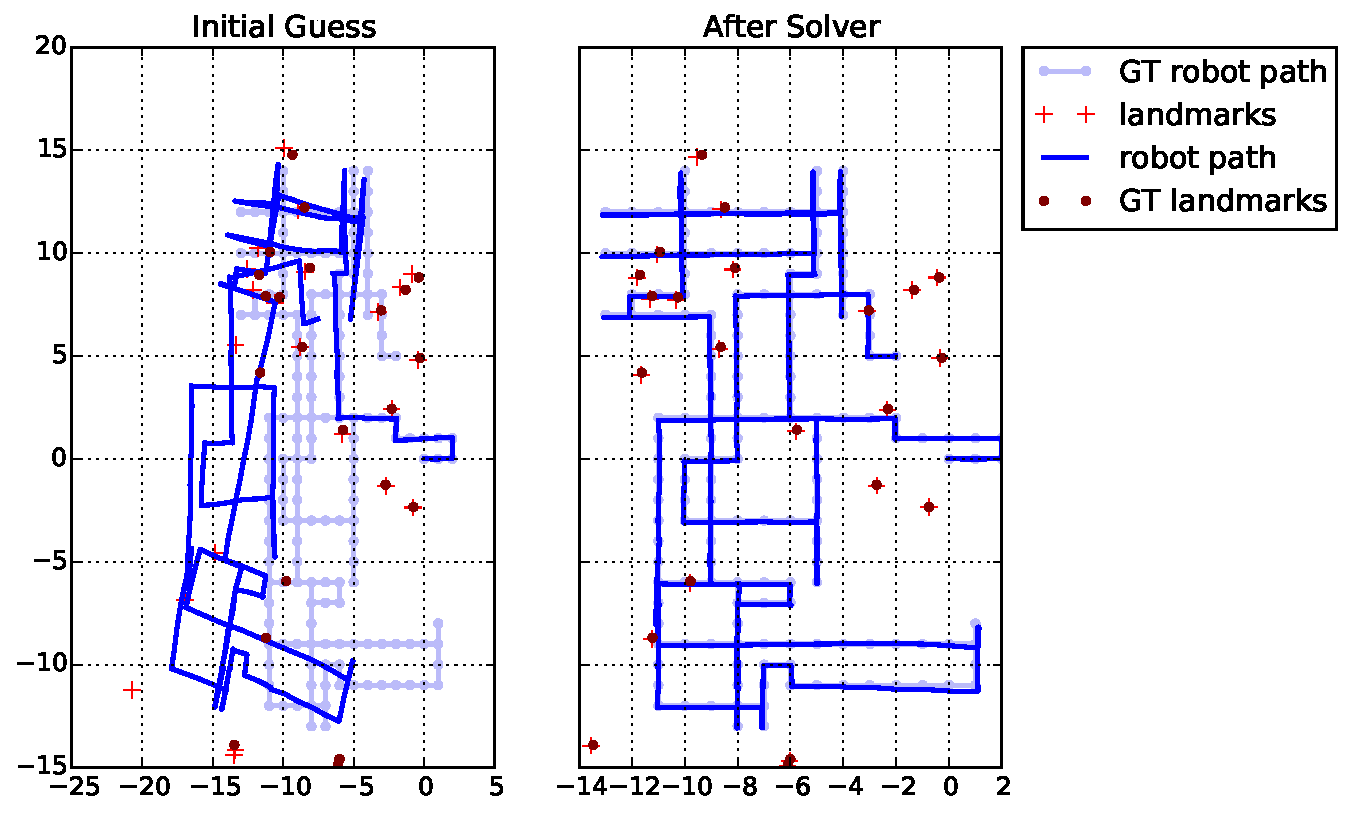
\includegraphics[width=\textwidth]{imagenes/tests/known/res_it_20_nl_40_op_1000_oa_1000_lp_1000_ds_300_kw_1.pdf}
\caption{Initial guess and solver estimation.}
\label{fig:test-ia}
\end{subfigure}\\
\begin{subfigure}[b]{\errorWidth\textwidth}
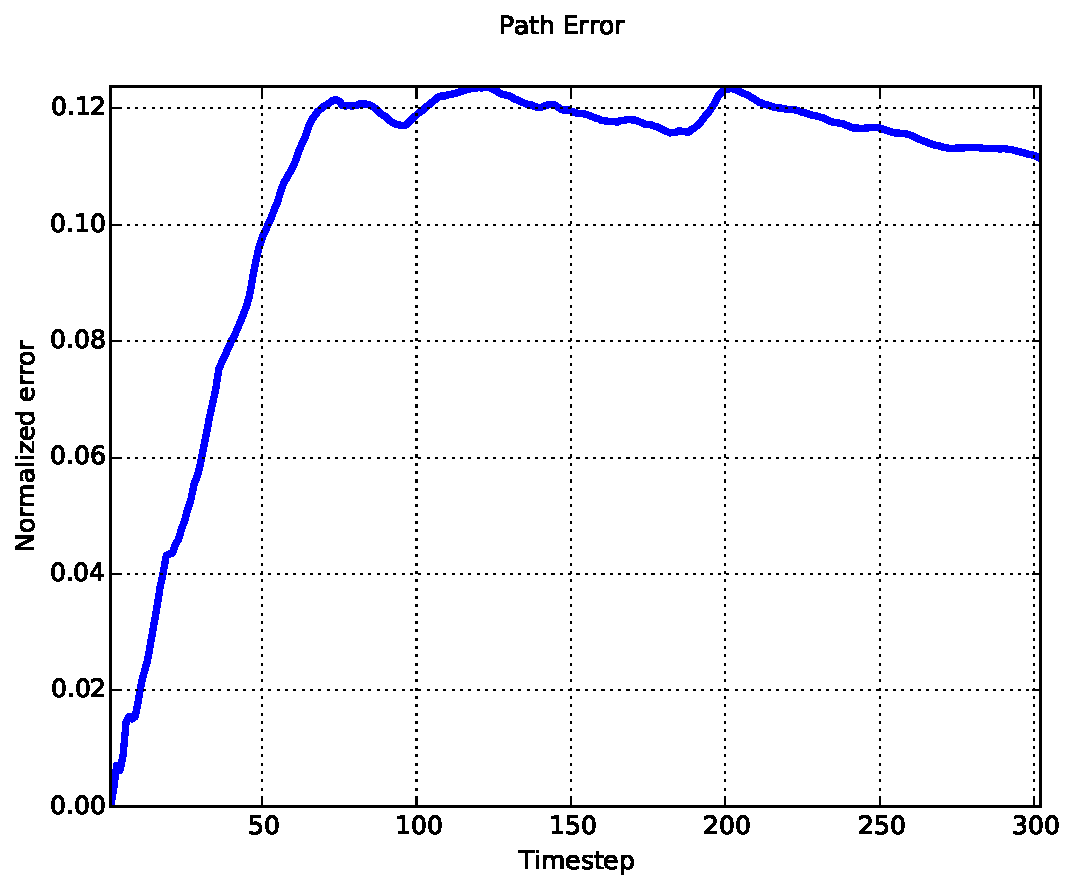
\includegraphics[width=\textwidth]{imagenes/tests/known/res_it_20_nl_40_op_1000_oa_1000_lp_1000_ds_300_kw_1_path.pdf}
\caption{Path normalized error.}
\label{fig:test-ib}
\end{subfigure}
\caption{Results for Test I.}
\label{fig:test-i}
\end{figure}
\clearpage

In the next test all the information parameters of the robot are decreased simultaneously. Is intended to show the effect in the estimation when adding uncertainty to the robot.

\nameref{sec:test-ii}, \nameref{sec:test-iii}, and \nameref{sec:test-iv}, shows the results when $i_{op}=i_{oa}=i_{lp}=100$, $i_{op}=i_{oa}=i_{lp}=10$, and $i_{op}=i_{oa}=i_{lp}=1$ respectively.

%It can be seen that the algorithm can retrieve the path with relative success when the information is 100 and 10, even when the initial guess is very far off. Only when the information is 1, the algorithm breaks.

It can be seen that the estimated path gradually degrades as the the information decrease. Finally when the information is 1, the algorithm breaks.

\subsubsection{Test II}
\label{sec:test-ii}

\begin{table}[htbp!]
    \centering
    \begin{tabular}{|c|c|c|c|c|c|c|}
        \hline
        $n_p$ & $n_l$ & $i_{op}$ & $i_{oa}$ & $i_{lp}$ & $it$ & $k_w$\\
        \hline \hline
        300 & 40 & 100 & 100 & 100 & 20 & 1\\
        \hline 
    \end{tabular}
    \caption{Parameters for Test II.}
    \label{tab:test-ii}
\end{table}

\begin{figure}[htbp!]
    \centering
    \begin{subfigure}[b]{\estWidth\textwidth}
        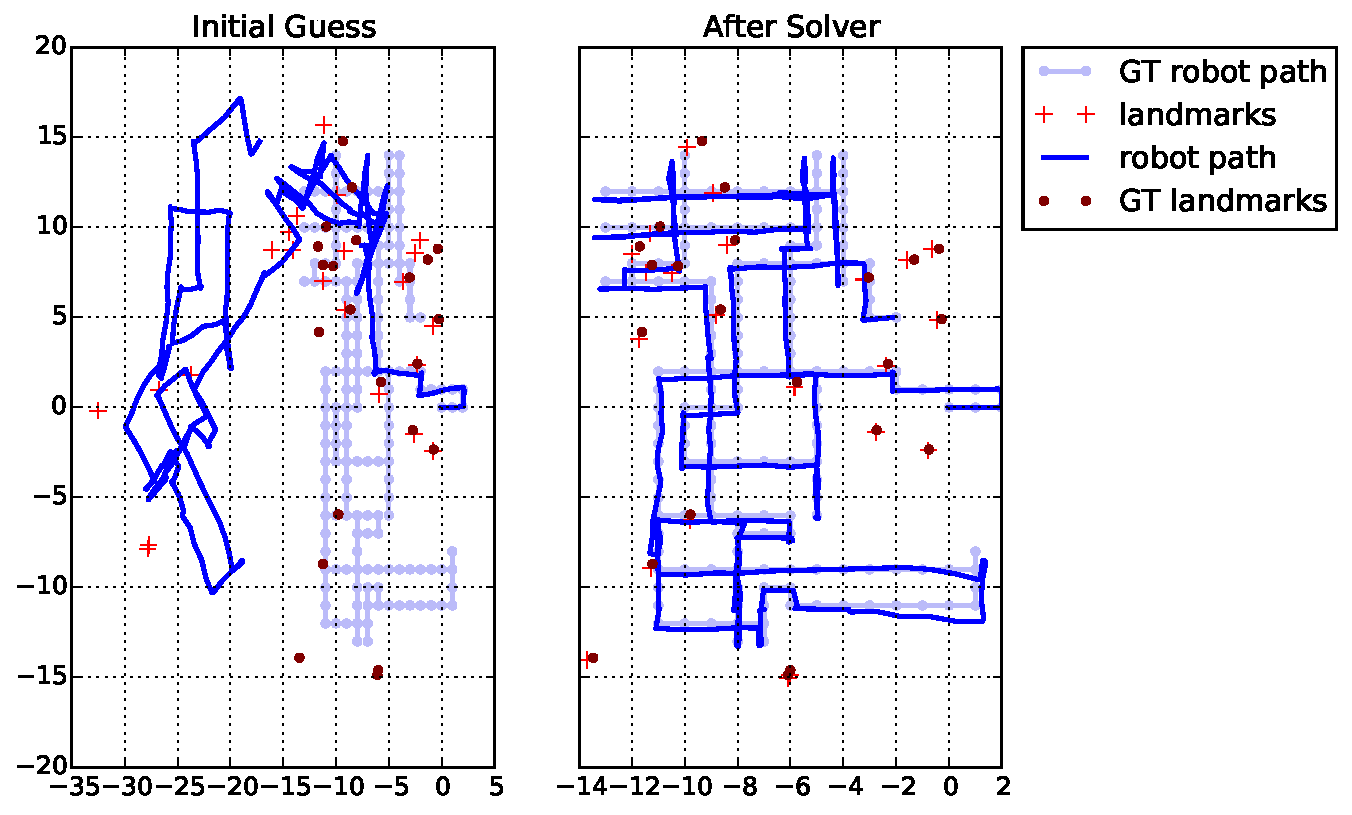
\includegraphics[width=\textwidth]{imagenes/tests/known/res_it_20_nl_40_op_100_oa_100_lp_100_ds_300_kw_1.pdf}
        \caption{Initial guess and solver estimation.}
        \label{fig:test-iia}
    \end{subfigure}\\
    \begin{subfigure}[b]{\errorWidth\textwidth}
        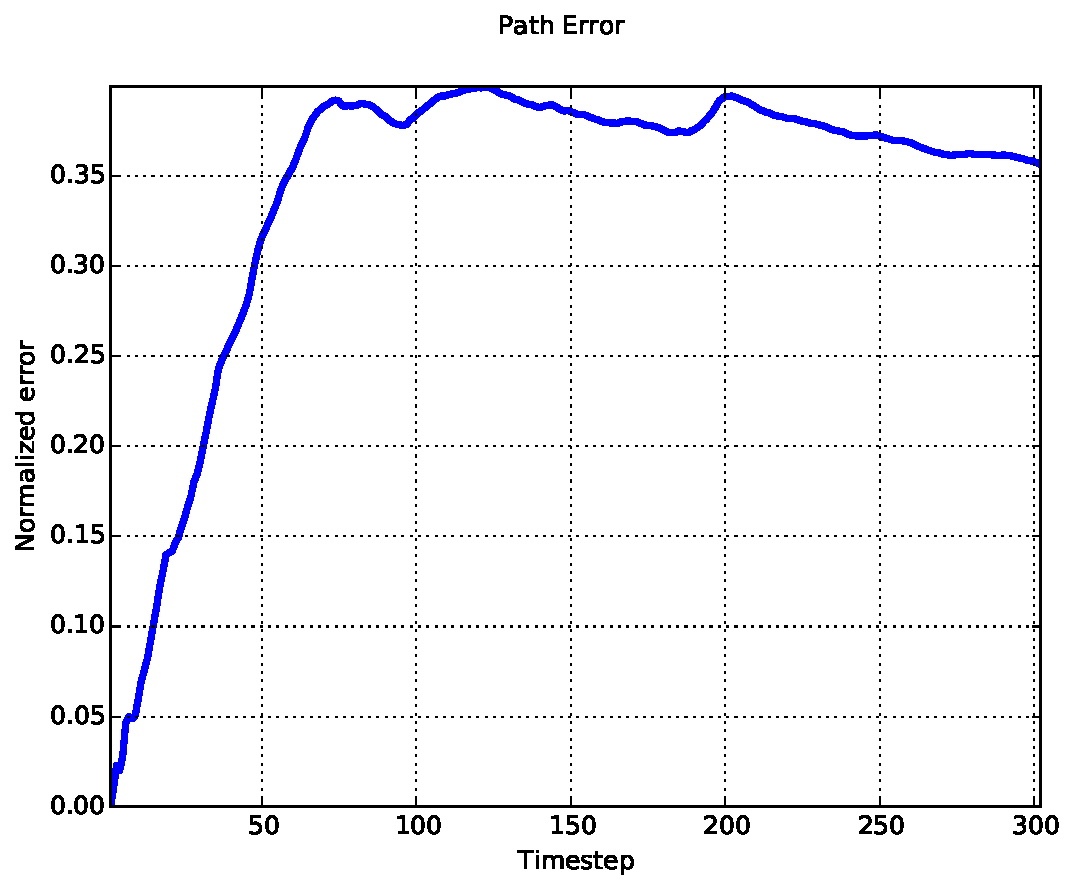
\includegraphics[width=\textwidth]{imagenes/tests/known/res_it_20_nl_40_op_100_oa_100_lp_100_ds_300_kw_1_path.pdf}
        \caption{Path normalized error.}
        \label{fig:test-iib}
    \end{subfigure}
    \caption{Results for Test II.}
    \label{fig:test-ii}
\end{figure}
\clearpage

\subsubsection{Test III}
\label{sec:test-iii}

\begin{table}[htbp!]
    \centering
    \begin{tabular}{|c|c|c|c|c|c|c|}
        \hline
        $n_p$ & $n_l$ & $i_{op}$ & $i_{oa}$ & $i_{lp}$ & $it$ & $k_w$\\
        \hline \hline
        300 & 40 & 10 & 10 & 10 & 20 & 1\\
        \hline 
    \end{tabular}
    \caption{Parameters for Test III.}
    \label{tab:test-iii}
\end{table}

\begin{figure}[htbp!]
    \centering
    \begin{subfigure}[b]{\estWidth\textwidth}
        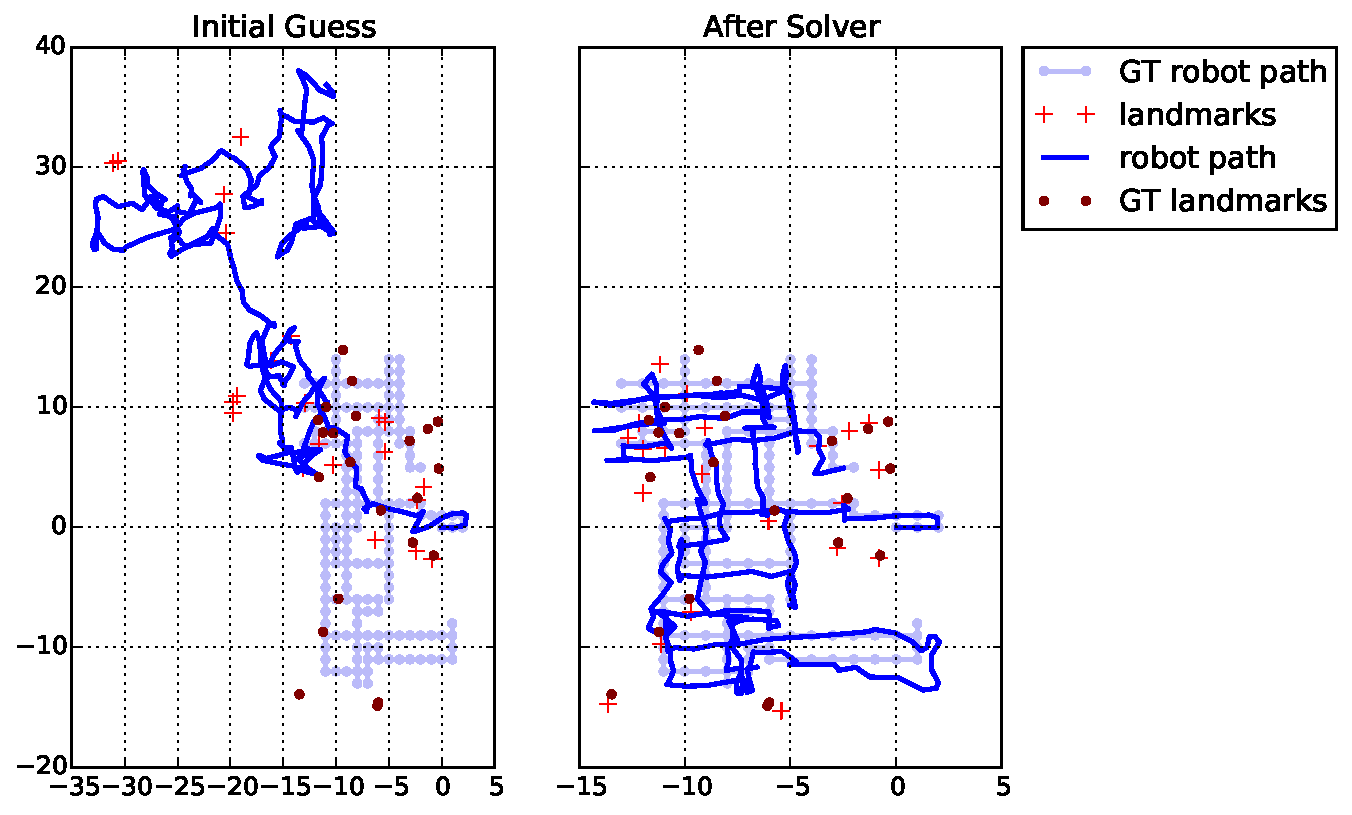
\includegraphics[width=\textwidth]{imagenes/tests/known/res_it_20_nl_40_op_10_oa_10_lp_10_ds_300_kw_1.pdf}
        \caption{Initial guess and solver estimation.}
        \label{fig:test-iiia}
    \end{subfigure}\\
    \begin{subfigure}[b]{\errorWidth\textwidth}
        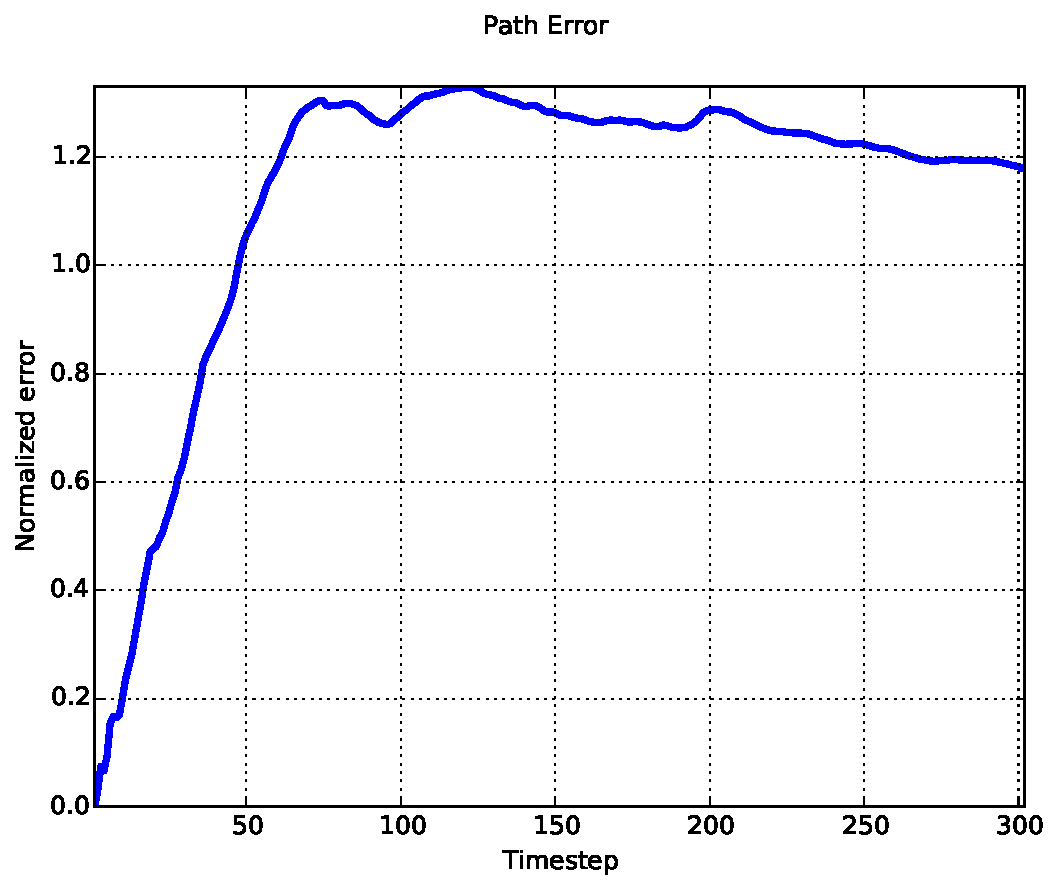
\includegraphics[width=\textwidth]{imagenes/tests/known/res_it_20_nl_40_op_10_oa_10_lp_10_ds_300_kw_1_path.pdf}
        \caption{Path normalized error.}
        \label{fig:test-iiib}
    \end{subfigure}
    \caption{Results for Test III.}
    \label{fig:test-iii}
\end{figure}
\clearpage

\subsubsection{Test IV}
\label{sec:test-iv}

\begin{table}[htbp!]
    \centering
    \begin{tabular}{|c|c|c|c|c|c|c|}
        \hline
        $n_p$ & $n_l$ & $i_{op}$ & $i_{oa}$ & $i_{lp}$ & $it$ & $k_w$\\
        \hline \hline
        300 & 40 & 1 & 1 & 1 & 20 & 1\\
        \hline 
    \end{tabular}
    \caption{Parameters for Test IV.}
    \label{tab:test-iv}
\end{table}

\begin{figure}[htbp!]
    \centering
    \begin{subfigure}[b]{\estWidth\textwidth}
        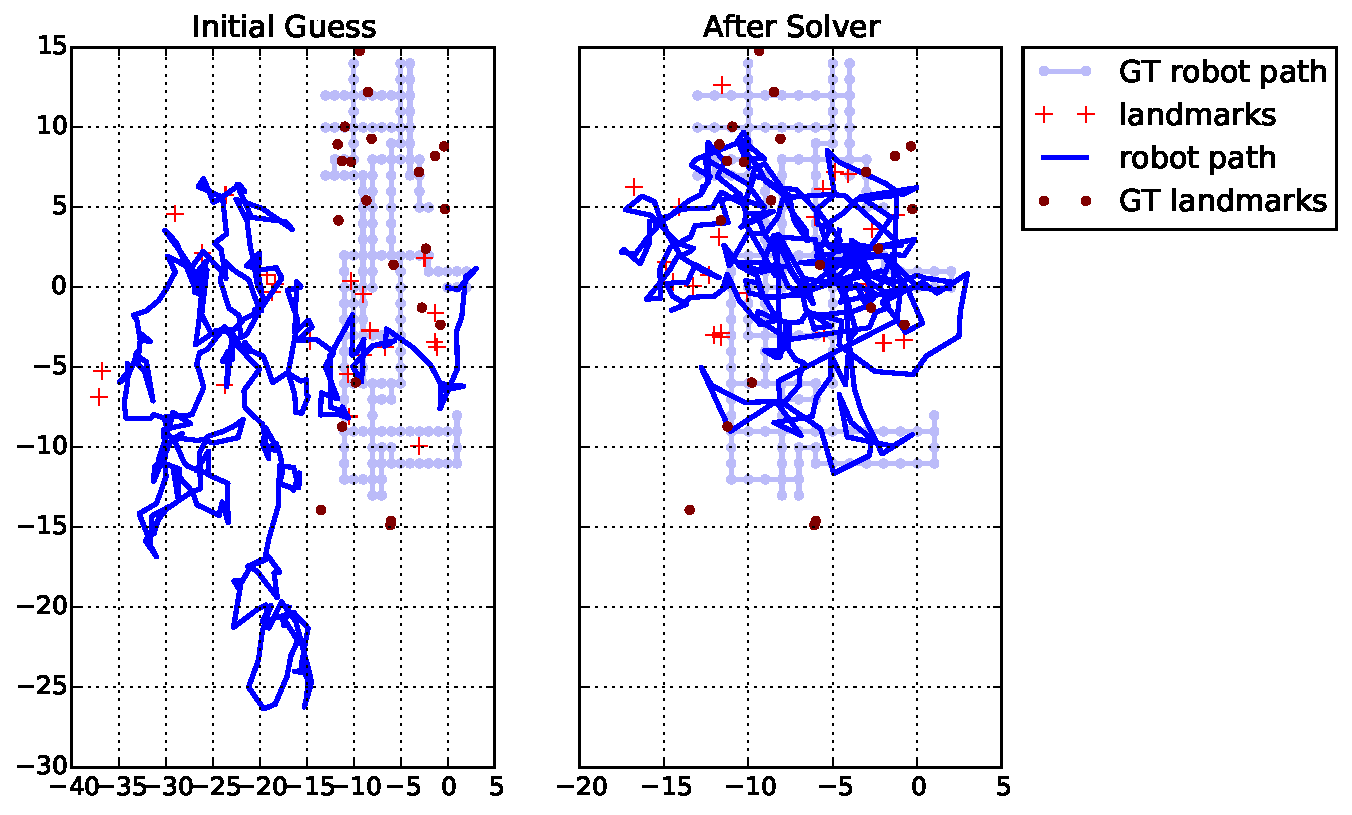
\includegraphics[width=\textwidth]{imagenes/tests/known/res_it_20_nl_40_op_1_oa_1_lp_1_ds_300_kw_1.pdf}
        \caption{Initial guess and solver estimation.}
        \label{fig:test-iva}
    \end{subfigure}\\
    \begin{subfigure}[b]{\errorWidth\textwidth}
        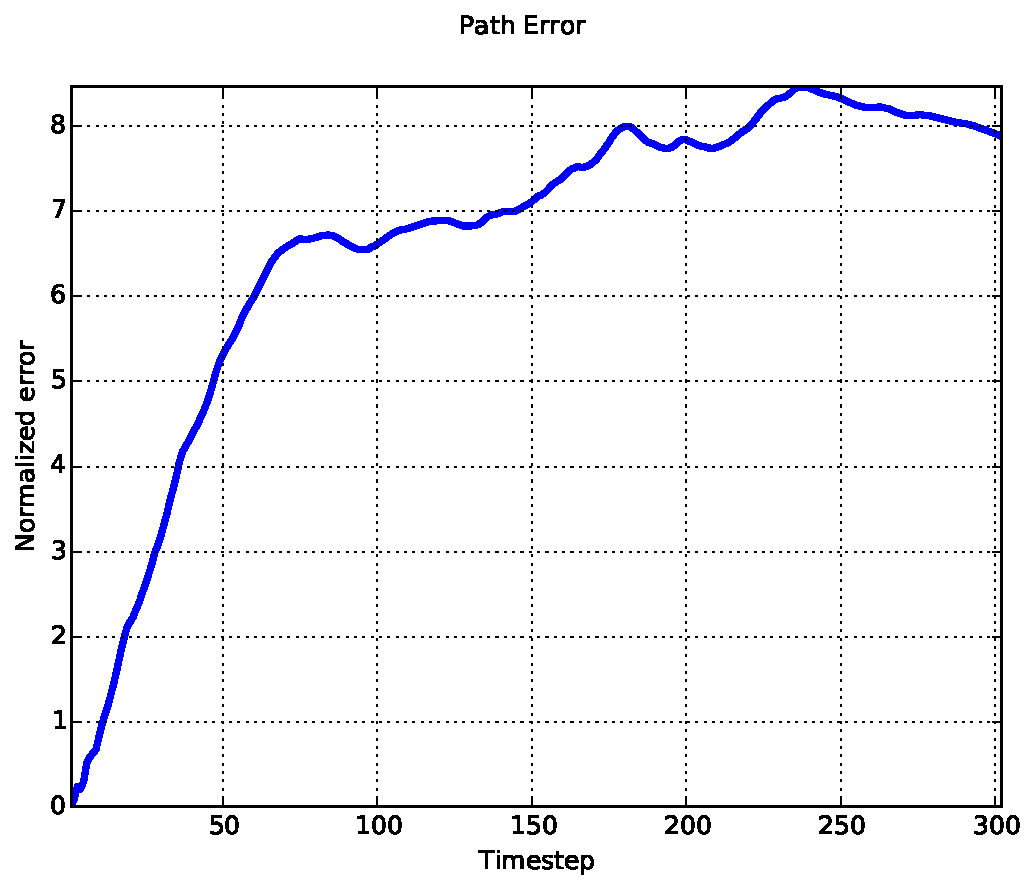
\includegraphics[width=\textwidth]{imagenes/tests/known/res_it_20_nl_40_op_1_oa_1_lp_1_ds_300_kw_1_path.pdf}
        \caption{Path normalized error.}
        \label{fig:test-ivb}
    \end{subfigure}
    \caption{Results for Test IV.}
    \label{fig:test-iv}
\end{figure}
\clearpage

\nameref{sec:test-v} shows the effect running the algorithm with a low number of iterations. In this case $it=1$. It can be seen that the algorithm was not able to converge properly, in contrast to~\nameref{sec:test-i}.

\subsubsection{Test V.}
\label{sec:test-v}

\begin{table}[htbp!]
    \centering
    \begin{tabular}{|c|c|c|c|c|c|c|}
        \hline
        $n_p$ & $n_l$ & $i_{op}$ & $i_{oa}$ & $i_{lp}$ & $it$ & $k_w$\\
        \hline \hline
        300 & 40 & 1000 & 1000 & 1000 & 1 & 1\\
        \hline 
    \end{tabular}
    \caption{Parameters for Test V.}
    \label{tab:test-v}
\end{table}

\begin{figure}[htbp!]
    \centering
    \begin{subfigure}[b]{\estWidth\textwidth}
        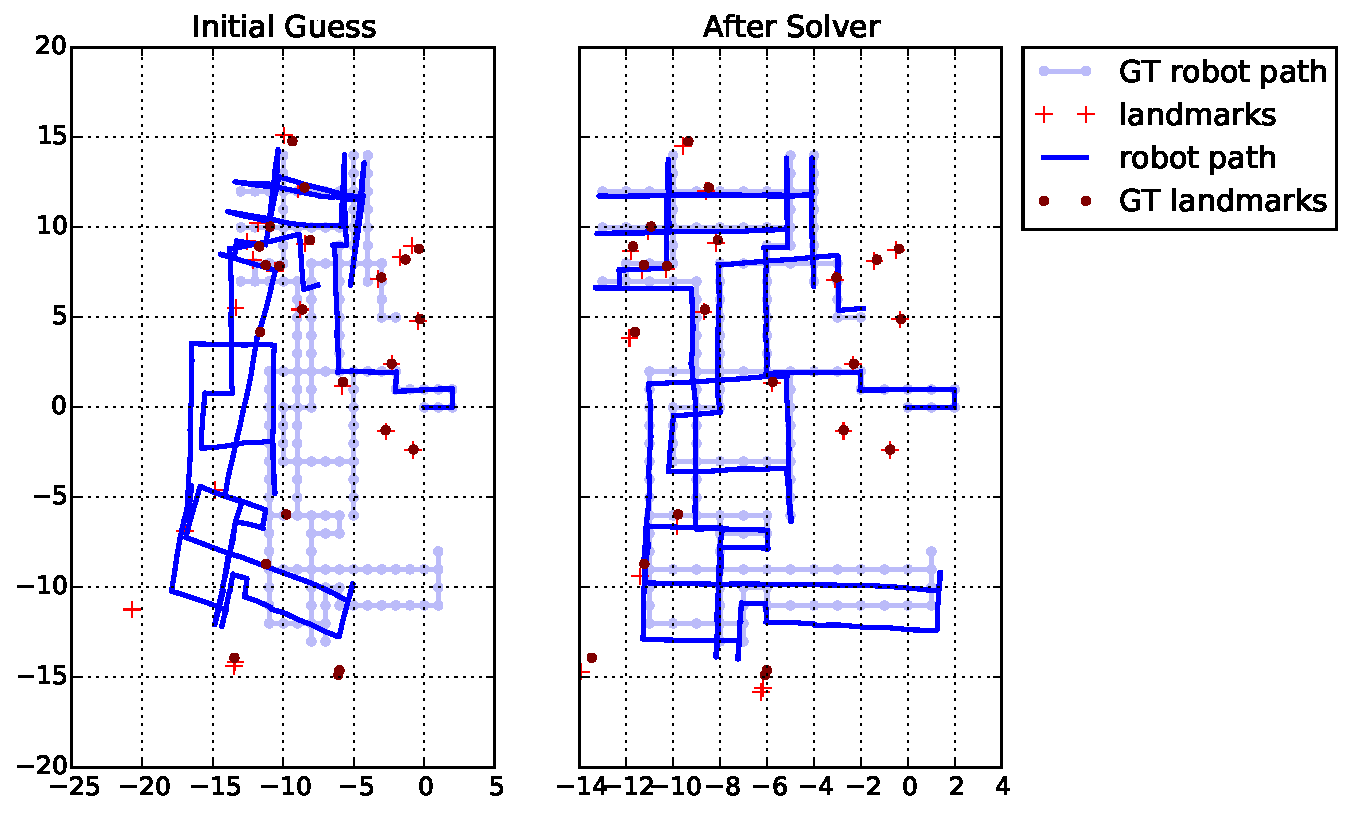
\includegraphics[width=\textwidth]{imagenes/tests/known/res_it_1_nl_40_op_1000_oa_1000_lp_1000_ds_300_kw_1.pdf}
        \caption{Initial guess and solver estimation.}
        \label{fig:test-va}
    \end{subfigure}\\
    \begin{subfigure}[b]{\errorWidth\textwidth}
        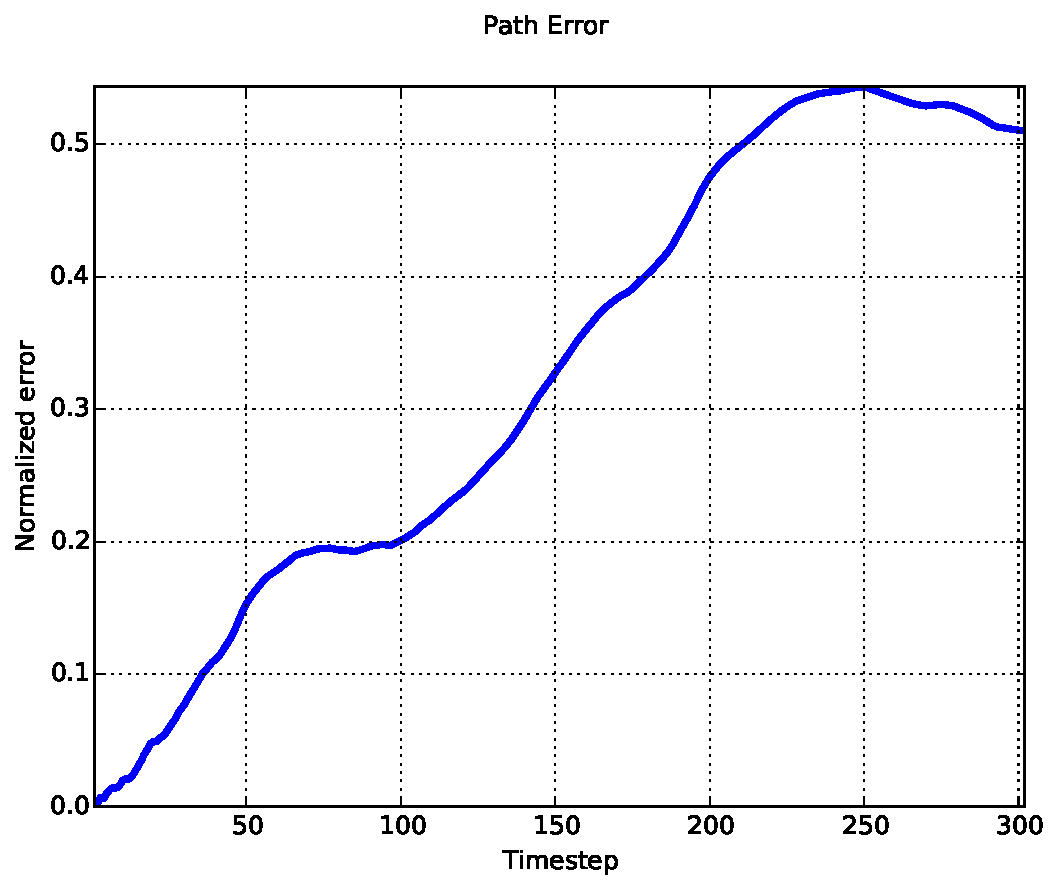
\includegraphics[width=\textwidth]{imagenes/tests/known/res_it_1_nl_40_op_1000_oa_1000_lp_1000_ds_300_kw_1_path.pdf}
        \caption{Path normalized error.}
        \label{fig:test-vb}
    \end{subfigure}
    \caption{Results for Test V.}
    \label{fig:test-v}
\end{figure}
\clearpage

In~\nameref{sec:test-vi} the kernel width was reduced to $k_w=0.1$, meaning that the effect of the kernel is applied earlier in distance. It can be seen that the new width actually improves the results, getting a normalized error for the full path of around 0.08.

\subsubsection{Test VI.}
\label{sec:test-vi}

\begin{table}[htbp!]
    \centering
    \begin{tabular}{|c|c|c|c|c|c|c|}
        \hline
        $n_p$ & $n_l$ & $i_{op}$ & $i_{oa}$ & $i_{lp}$ & $it$ & $k_w$\\
        \hline \hline
        300 & 40 & 1000 & 1000 & 1000 & 20 & 0.1\\
        \hline 
    \end{tabular}
    \caption{Parameters for Test VI.}
    \label{tab:test-vi}
\end{table}

\begin{figure}[htbp!]
    \centering
    \begin{subfigure}[b]{\estWidth\textwidth}
        \includegraphics[width=\textwidth]{imagenes/tests/known/{res_it_20_nl_40_op_1000_oa_1000_lp_1000_ds_300_kw_0.1}.pdf}
        \caption{Initial guess and solver estimation.}
        \label{fig:test-via}
    \end{subfigure}\\
    \begin{subfigure}[b]{\errorWidth\textwidth}
        \includegraphics[width=\textwidth]{imagenes/tests/known/{res_it_20_nl_40_op_1000_oa_1000_lp_1000_ds_300_kw_0.1_path}.pdf}
        \caption{Path normalized error.}
        \label{fig:test-vib}
    \end{subfigure}
    \caption{Results for Test VI.}
    \label{fig:test-vi}
\end{figure}
\clearpage

In terms of speed the algorithm performs quite fast, taking around $1[s]$ for all the tests.

\section{Unknown Data Association}
\label{sec:unknown-asso-res}

In this section similar tests are made, but in this case it is assumed unknown data association of the landmarks. The same simulator is used to generate the data, and Algorithm~\ref{alg:final} to compute the estimate.

Along with the parameters used in the known correspondence case, the following new parameters must be set in these tests:

\begin{itemize}
\item $\chi$: likelihood threshold for data association.
\item $dt$: maximum distance for distance test.
\item $io$: inter full optimization frequency.
\item $ps$: Pose skipping.
\end{itemize}

Where $\chi$ and $dt$ are the thresholds used in Algorithm~\ref{alg:incremental-data-association}. $io$ is the number of incremental optimization between two full optimizations, and $ps$ is the number of pose between optimizations, both form Algorithm~\ref{alg:final}.

\nameref{sec:test-vii} show the results for a successful test with unknown data association. Notice that in the initial guess there are several more landmarks that in the groundtruth. That is because the initial guess consider every single measurement as an independent landmark. However in the result of the solver, the algorithm is able to associate the the measurements with the corresponding landmark, and correct the path of the robot. Nevertheless there are 4 cases that is unable to associate correctly.

The parameter $dt$ is set to $\infty$ so no distant test is performed. In table~\ref{tab:test-vii}, variable $t$ correspond to the total time of the algorithm. 

\subsubsection{Test VII.}
\label{sec:test-vii}

\begin{table}[htbp!]
    \centering
    \begin{tabular}{|c|c|c|c|c|c|c|c|c|c|c|c|}
        \hline
        $n_p$ & $n_l$ & $i_{op}$ & $i_{oa}$ & $i_{lp}$ & $it$ & $k_w$ & $\chi$ & $dt$ & $io$ & $ps$ & $t$\\
        \hline \hline
        400 & 30 & 1000 & 10000 & 1000 & 20 & 1 & 0.1 & $\infty$ & 400 & 10 & $13[s]$\\
        \hline 
    \end{tabular}
    \caption{Parameters for Test VII.}
    \label{tab:test-vii}
\end{table}

\begin{figure}[htbp!]
    \centering
    \begin{subfigure}[b]{\estWidth\textwidth}
        \includegraphics[width=\textwidth]{imagenes/tests/unknown/{res_it_20_xi_0.1_nl_30_op_1000_oa_10000_lp_1000_dsk_1_io_400_ds_400_dt_0_kw_1_ps_10}.pdf}
        \caption{Initial guess and solver estimation.}
        \label{fig:test-viia}
    \end{subfigure}\\
    \begin{subfigure}[b]{\errorWidth\textwidth}
        \includegraphics[width=\textwidth]{imagenes/tests/unknown/{res_it_20_xi_0.1_nl_30_op_1000_oa_10000_lp_1000_dsk_1_io_400_ds_400_dt_0_kw_1_ps_10_path}.pdf}
        \caption{Path normalized error.}
        \label{fig:test-viib}
    \end{subfigure}
    \caption{Results for Test VII.}
    \label{fig:test-vii}
\end{figure}
\clearpage

In the next tests the threshold $\chi$ is modified. In~\nameref{sec:test-viii} the threshold is set to a very low value $\chi=10^{-100}$. It can be seen that the algorithm merge non equivalent landmarks, which make the estimated path to breaks.
In~\nameref{sec:test-ix} and \nameref{sec:test-x} $\chi$ is set to 1 and 3 respectively. In these cases the thresholds are so high that the algorithm is unable to associate all the equivalent landmarks. This cause that the estimated path gradually drift.

\subsubsection{Test VIII.}
\label{sec:test-viii}

\begin{table}[htbp!]
    \centering
    \begin{tabular}{|c|c|c|c|c|c|c|c|c|c|c|c|}
        \hline
        $n_p$ & $n_l$ & $i_{op}$ & $i_{oa}$ & $i_{lp}$ & $it$ & $k_w$ & $\chi$ & $dt$ & $io$ & $ps$ & $t$\\
        \hline \hline
        400 & 30 & 1000 & 10000 & 1000 & 20 & 1 & $10^{-100}$ & $\infty$ & 400 & 10 & $94[s]$\\
        \hline 
    \end{tabular}
    \caption{Parameters for Test VIII.}
    \label{tab:test-viii}
\end{table}

\begin{figure}[htbp!]
    \centering
    \begin{subfigure}[b]{\estWidth\textwidth}
        \includegraphics[width=\textwidth]{imagenes/tests/unknown/{res_it_20_xi_1e-100_nl_30_op_1000_oa_10000_lp_1000_dsk_1_io_400_ds_400_dt_0_kw_1_ps_10}.pdf}
        \caption{Initial guess and solver estimation.}
        \label{fig:test-viiia}
    \end{subfigure}\\
    \begin{subfigure}[b]{\errorWidth\textwidth}
        \includegraphics[width=\textwidth]{imagenes/tests/unknown/{res_it_20_xi_1e-100_nl_30_op_1000_oa_10000_lp_1000_dsk_1_io_400_ds_400_dt_0_kw_1_ps_10_path}.pdf}
        \caption{Path normalized error.}
        \label{fig:test-viiib}
    \end{subfigure}
    \caption{Results for Test VIII.}
    \label{fig:test-viii}
\end{figure}
\clearpage

\subsubsection{Test IX.}
\label{sec:test-ix}

\begin{table}[htbp!]
    \centering
    \begin{tabular}{|c|c|c|c|c|c|c|c|c|c|c|c|}
        \hline
        $n_p$ & $n_l$ & $i_{op}$ & $i_{oa}$ & $i_{lp}$ & $it$ & $k_w$ & $\chi$ & $dt$ & $io$ & $ps$ & $t$\\
        \hline \hline
        400 & 30 & 1000 & 10000 & 1000 & 20 & 1 & 1 & $\infty$ & 400 & 10 & $10[s]$\\
        \hline 
    \end{tabular}
    \caption{Parameters for Test IX.}
    \label{tab:test-ix}
\end{table}

\begin{figure}[htbp!]
    \centering
    \begin{subfigure}[b]{\estWidth\textwidth}
        \includegraphics[width=\textwidth]{imagenes/tests/unknown/{res_it_20_xi_1_nl_30_op_1000_oa_10000_lp_1000_dsk_1_io_400_ds_400_dt_0_kw_1_ps_10}.pdf}
        \caption{Initial guess and solver estimation.}
        \label{fig:test-ixa}
    \end{subfigure}\\
    \begin{subfigure}[b]{\errorWidth\textwidth}
        \includegraphics[width=\textwidth]{imagenes/tests/unknown/{res_it_20_xi_1_nl_30_op_1000_oa_10000_lp_1000_dsk_1_io_400_ds_400_dt_0_kw_1_ps_10_path}.pdf}
        \caption{Path normalized error.}
        \label{fig:test-ixb}
    \end{subfigure}
    \caption{Results for Test IX.}
    \label{fig:test-ix}
\end{figure}
\clearpage

\subsubsection{Test X.}
\label{sec:test-x}

\begin{table}[htbp!]
    \centering
    \begin{tabular}{|c|c|c|c|c|c|c|c|c|c|c|c|}
        \hline
        $n_p$ & $n_l$ & $i_{op}$ & $i_{oa}$ & $i_{lp}$ & $it$ & $k_w$ & $\chi$ & $dt$ & $io$ & $ps$ & $t$\\
        \hline \hline
        400 & 30 & 1000 & 10000 & 1000 & 20 & 1 & 3 & $\infty$ & 400 & 10 & $17[s]$\\
        \hline 
    \end{tabular}
    \caption{Parameters for Test X.}
    \label{tab:test-x}
\end{table}

\begin{figure}[htbp!]
    \centering
    \begin{subfigure}[b]{\estWidth\textwidth}
        \includegraphics[width=\textwidth]{imagenes/tests/unknown/{res_it_20_xi_3_nl_30_op_1000_oa_10000_lp_1000_dsk_1_io_400_ds_400_dt_0_kw_1_ps_10}.pdf}
        \caption{Initial guess and solver estimation.}
        \label{fig:test-xa}
    \end{subfigure}\\
    \begin{subfigure}[b]{\errorWidth\textwidth}
        \includegraphics[width=\textwidth]{imagenes/tests/unknown/{res_it_20_xi_3_nl_30_op_1000_oa_10000_lp_1000_dsk_1_io_400_ds_400_dt_0_kw_1_ps_10_path}.pdf}
        \caption{Path normalized error.}
        \label{fig:test-xb}
    \end{subfigure}
    \caption{Results for Test X.}
    \label{fig:test-x}
\end{figure}
\clearpage

In~\nameref{sec:test-xi} $\chi$ gets the value of $\infty$ and $dt=1$, so that in this case the algorithm associate landmarks using the distant test instead of the correspondence test. Every landmark at a distance of 1 unit will be automatically associated. Looking at Figure~\ref{fig:test-xia} it can be seen that now all landmarks are correctly associated. However Figure~\ref{fig:test-xib} shows that the estimation has a greater cumulative error. Also, the distant test is faster than the correspondence test, taking only $5[s]$. Therefore a trade-off exists between using the distant test and the correspondence test as a mean to solve unknown association.

\subsubsection{Test XI.}
\label{sec:test-xi}

\begin{table}[htbp!]
    \centering
    \begin{tabular}{|c|c|c|c|c|c|c|c|c|c|c|c|}
        \hline
        $n_p$ & $n_l$ & $i_{op}$ & $i_{oa}$ & $i_{lp}$ & $it$ & $k_w$ & $\chi$ & $dt$ & $io$ & $ps$ & $t$\\
        \hline \hline
        400 & 30 & 1000 & 10000 & 1000 & 20 & 1 & $\infty$ & 1 & 400 & 10 & $5[s]$\\
        \hline 
    \end{tabular}
    \caption{Parameters for Test XI.}
    \label{tab:test-xi}
\end{table}

\begin{figure}[htbp!]
    \centering
    \begin{subfigure}[b]{\estWidth\textwidth}
        \includegraphics[width=\textwidth]{imagenes/tests/unknown/{res_it_20_xi_0_nl_30_op_1000_oa_10000_lp_1000_dsk_1_io_400_ds_400_dt_1_kw_1_ps_10}.pdf}
        \caption{Initial guess and solver estimation.}
        \label{fig:test-xia}
    \end{subfigure}\\
    \begin{subfigure}[b]{\errorWidth\textwidth}
        \includegraphics[width=\textwidth]{imagenes/tests/unknown/{res_it_20_xi_0_nl_30_op_1000_oa_10000_lp_1000_dsk_1_io_400_ds_400_dt_1_kw_1_ps_10_path}.pdf}
        \caption{Path normalized error.}
        \label{fig:test-xib}
    \end{subfigure}
    \caption{Results for Test XI.}
    \label{fig:test-xi}
\end{figure}
\clearpage

In~\nameref{sec:test-xii} the pose skip parameter is increase to $ps=100$. the idea is to do as least optimization as possible to increase the algorithm speed. It can be seen however that, due to the lack of optimization, the algorithm is unable to correct the path and to associate the landmarks. This errors also cause that the algorithm actually takes longer than in~\nameref{sec:test-vii}. 

\subsubsection{Test XII.}
\label{sec:test-xii}

\begin{table}[htbp!]
    \centering
    \begin{tabular}{|c|c|c|c|c|c|c|c|c|c|c|c|}
        \hline
        $n_p$ & $n_l$ & $i_{op}$ & $i_{oa}$ & $i_{lp}$ & $it$ & $k_w$ & $\chi$ & $dt$ & $io$ & $ps$ & $t$\\
        \hline \hline
        400 & 30 & 1000 & 10000 & 1000 & 20 & 1 & 0.1 & $\infty$ & 400 & 100 & $21[s]$\\
        \hline 
    \end{tabular}
    \caption{Parameters for Test XII.}
    \label{tab:test-xii}
\end{table}

\begin{figure}[htbp!]
    \centering
    \begin{subfigure}[b]{\estWidth\textwidth}
        \includegraphics[width=\textwidth]{imagenes/tests/unknown/{res_it_20_xi_0.1_nl_30_op_1000_oa_10000_lp_1000_dsk_1_io_400_ds_400_dt_0_kw_1_ps_100}.pdf}
        \caption{Initial guess and solver estimation.}
        \label{fig:test-xiia}
    \end{subfigure}\\
    \begin{subfigure}[b]{\errorWidth\textwidth}
        \includegraphics[width=\textwidth]{imagenes/tests/unknown/{res_it_20_xi_0.1_nl_30_op_1000_oa_10000_lp_1000_dsk_1_io_400_ds_400_dt_0_kw_1_ps_100_path}.pdf}
        \caption{Path normalized error.}
        \label{fig:test-xiib}
    \end{subfigure}
    \caption{Results for Test XII.}
    \label{fig:test-xii}
\end{figure}
\clearpage
 
\section{Real Data}
\label{sec:real-data-res} 

In this section the correctness of the algorithm is proven for more realistic data. The size of the data is much larger than the previous cases, the number of poses in a path are in the order of thousands and ten thousands. Unfortunately the amount of data is so large, that it becomes infeasible to apply the correspondence test. For this reason, only the distant test is used. Moreover, the data presents undesired properties like non-Gaussian noise and false alarms, nevertheless it'll be shown that it's still possible to apply the algorithm and get good results.

\subsection{Husky a200 Robot}

The first of these test is a Husky a200 Robot simulated in Gazebo. Since this test is still a simulation the groundtruth and the path error can still be retrieved. However, since Gazebo is a more realistic simulation, the nonlinear models of the robot, miss in the detections and false alarms are also simulated. 

The parameters of the algorithm are presented it Table~\ref{tab:test-xii}. In this case the information parameters $i_{op}$, $i_{oa}$, and $i_{lp}$ are the assumed uncertainty that better fit the robot model. Since no knowledge was acquired about the robot, these parameters were chosen by trial and error. 

The result are shown in Figure~\ref{fig:test-xiii}. It can be seen that the algorithm can correctly predict the robot path. Most of the landmarks are also found, but there a lot of false positives, possibly generated by sensor malfunctions, spurious measurements, or moving objects. A possible way to get rid of these false alarms is to apply a policy of elimination of landmarks if they aren't measured a certain number of times. Nevertheless, the false alarms don't affect greatly the results of the estimation.

\subsubsection{Test XIII.}
\label{sec:test-xiii}

\begin{table}[htbp!]
    \centering
    \begin{tabular}{|c|c|c|c|c|c|c|c|c|c|c|c|}
        \hline
        $n_p$ & $n_l$ & $i_{op}$ & $i_{oa}$ & $i_{lp}$ & $it$ & $k_w$ & $\chi$ & $dt$ & $io$ & $ps$ & $t$\\
        \hline \hline
        4700 & 18 & 10000 & 10000 & 1000 & 10 & 1 & $\infty$ & 0.5 & 500 & 10 & $3[min]$\\
        \hline 
    \end{tabular}
    \caption{Parameters for Test XIII.}
    \label{tab:test-xiii}
\end{table}

\begin{figure}[htbp!]
    \centering
    \begin{subfigure}[b]{\estWidth\textwidth}
        \includegraphics[width=\textwidth]{imagenes/tests/real/{res_ROS_2015-12-11 19:29:05_it_10_xi_0_op_10000_oa_10000_lp_1000_dsk_1_io_500_ds_100000_dt_0.5_kw_1_ps_10}.pdf}
        \caption{Initial guess and solver estimation.}
        \label{fig:test-xiiia}
    \end{subfigure}\\
    \begin{subfigure}[b]{\errorWidth\textwidth}
        \includegraphics[width=\textwidth]{imagenes/tests/real/{res_ROS_2015-12-11 19:29:05_it_10_xi_0_op_10000_oa_10000_lp_1000_dsk_1_io_500_ds_100000_dt_0.5_kw_1_ps_10_path}.pdf}
        \caption{Path normalized error.}
        \label{fig:test-xiiib}
    \end{subfigure}
    \caption{Results for Test XIII.}
    \label{fig:test-xiii}
\end{figure}
\clearpage

\subsection{Parque O'Higgins}

This dataset correspond to data taken in Parque O'Higgins by a robot from Universidad de Chile. Since this is real data there is no groundtruth with which compare the results. However, the robot was controlled so that it return to the starting position at the end of the path, so it's possible to check the correctness of the algorithm by looking at the robot's final position. Also, since there is no groudtruth there no way to known the correct amount to landmarks in the map.

The results are shown in~\nameref{sec:test-xiv}, along with the parameters used in the test. It can be seen that in the initial guess the robot doesn't return to the starting position (0,0), however it does when the algorithm is applied, thus proving the correctness of the estimate. Due to the large size of the data the algorithm took 4 hours to finish.


\subsubsection{Test XIV.}
\label{sec:test-xiv}

\begin{table}[htbp!]
    \centering
    \begin{tabular}{|c|c|c|c|c|c|c|c|c|c|c|c|}
        \hline
        $n_p$ & $n_l$ & $i_{op}$ & $i_{oa}$ & $i_{lp}$ & $it$ & $k_w$ & $\chi$ & $dt$ & $io$ & $ps$ & $t$\\
        \hline \hline
        8130 & - & 100000 & 100000 & 100 & 10 & 1 & $\infty$ & 3 & 500 & 10 & $4[hrs]$\\
        \hline 
    \end{tabular}
    \caption{Parameters for Test XIV.}
    \label{tab:test-xiv}
\end{table}

\begin{figure}[htbp!]
    \centering
    \includegraphics[width=\estWidth\textwidth]{imagenes/tests/real/{res_ohiggins_2015-12-11 23:49:28_it_10_xi_0_op_100000_oa_100000_lp_100_dsk_1_io_500_ds_100000_dt_3_kw_1_ps_10}.pdf}
    \caption{Results for Test XIV.}
    \label{fig:test-xiv}
\end{figure}
\todo[inline]{add park background}
\clearpage

\subsection{Victoria Park}

The Victoria Park\footnote{Avaliable in \url{http://www.mrpt.org/Dataset_The_Victoria_Park}} is as commonly used datatest to test algorithms related to localization, mapping and SLAM. Again no real groundtruth of the data exist, however in this case the results can be compared with ones obtained by similar algorithms. 

\nameref{sec:test-xv} show the results of the algorithm in the Victoria Park dataset. In Figure~\ref{fig:victoria-isam} the results for the same dataset are presented, using the iSAM algorithm~\cite{isam}. It can be appreciated the resemblance between the two results. The mayor difference is the number of landmarks, since this implementation of GraphSLAM doesn't have a way to eliminate false alarms, they will stay forever in the map. The mayor disadvantage of the GraphSLAM algorithm is the computation time, due to the size of the dataset, it took 10 hours to finish.

\subsubsection{Test XV.}
\label{sec:test-xv}

\begin{table}[htbp!]
    \centering
    \begin{tabular}{|c|c|c|c|c|c|c|c|c|c|c|c|}
        \hline
        $n_p$ & $n_l$ & $i_{op}$ & $i_{oa}$ & $i_{lp}$ & $it$ & $k_w$ & $\chi$ & $dt$ & $io$ & $ps$ & $t$\\
        \hline \hline
        61763 & - & 8000 & 100000 & 5 & 15 & 1 & $\infty$ & 5 & 500 & 10 & $10[hrs]$\\
        \hline 
    \end{tabular}
    \caption{Parameters for Test XV.}
    \label{tab:test-xv}
\end{table}

\begin{figure}[htbp!]
    \centering
    \includegraphics[width=\estWidth\textwidth]{imagenes/tests/real/{res_victoria_2015-12-14 01:28:19_it_15_xi_0_op_8000_oa_100000_lp_5_dsk_1_io_500_ds_100000_dt_5_kw_1_ps_10}.pdf}
    \caption{Results for Test XV.}
    \label{fig:test-xv}
\end{figure}
\todo[inline]{add park background}
\clearpage

\begin{figure}[htbp!]
    \centering
    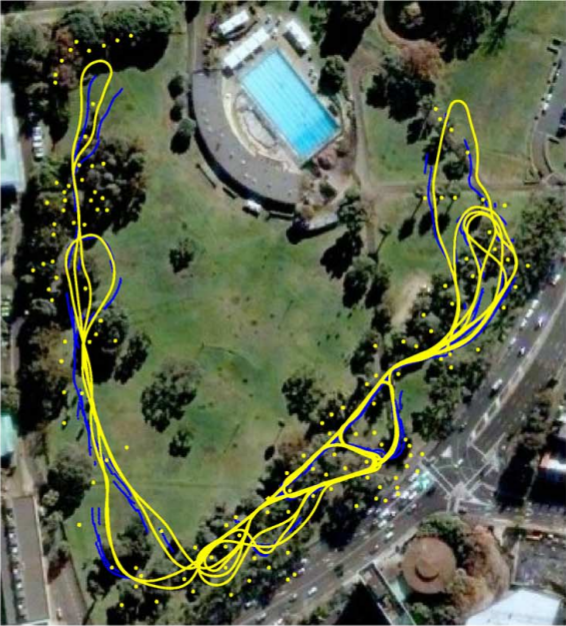
\includegraphics[width=0.5\textwidth]{imagenes/victoria-isam.png}
    \caption{Results iSAM in the Victoria Park dataset~\cite{isam}.}
    \label{fig:victoria-isam}
\end{figure}